\documentclass{report}
\usepackage{graphicx}
\usepackage{indentfirst}
\usepackage[OT1,T1]{fontenc}
\usepackage[french]{babel}
\usepackage{sidecap}
\usepackage{geometry}
\geometry{hmargin=2.5cm,vmargin=1.5cm}
\renewcommand{\thesection}{\arabic{section}}
\bibliographystyle{unsrt}

\begin{document}

\begin{titlepage}

\newcommand{\reportyear}{Avril 2024}
\newcommand{\HRule}{\rule{\linewidth}{0.5mm}} % Defines a new command for the horizontal lines, change thickness here
\center % Center everything on the page

\includegraphics[scale=0.3]{Images/logo_ub.png}\\[0,5cm] % Include a department/university logo - this will require the graphicx package

\includegraphics[scale=0.4]{Images/logo_inrae.PNG}\\[1cm] % Include a department/university logo - this will require the graphicx package
\textsc{\Large Conception d'un projet de recherche et de développement}\\[0.5cm] % Major heading such as course name
\HRule \\[0.4cm]
{ \huge \bfseries Cahier des charges du projet : Analyse de données RNA-Seq (champignons \textit{Fusarium})}\\[0.3cm] % Title of your document
\HRule \\[0,8cm]
% If you don't want a supervisor, uncomment the two lines below and remove the section above

\Large \emph{Clients:}\\
Nadia \textsc{Ponts}\\
Fabien \textsc{Dumetz}\\[0,8cm]

\Large \emph{Laboratoire:}\\
L’Institut National de Recherche pour l’Agriculture, l’Alimentation et l’Environnement\\[0,8cm]

\Large \emph{Auteurs:}\\
Djemilatou \textsc{Ouandaogo}\\
Linda \textsc{Khodja}\\
Lucien \textsc{Piat}\\
Maroa \textsc{Alani}\\[0,8cm]

\Large \emph{Superviseur:}\\
 Marie \textsc{Beurton-Aimar}\\[1cm]
\reportyear

\vfill % Fill the rest of the page with whitespace
\end{titlepage}

\tableofcontents

\newpage

\chapter{Introduction}

L'INRAE, ou Institut National de Recherche pour l'Agriculture, l'Alimentation et l'Environnement, est un organisme public de recherche français. En son sein,  l’unité de recherche Mycologie et Sécurité des Aliments cherche à comprendre les mécanismes de contamination des aliments par les mycotoxines. \cite{inrae} \\

Les champignons du genre \textit{Fusarium} infectent le blé et produisent des toxines sur les épis destinés à la consommation. Ces derniers élevés en co-culture forment un Meta-organisme, le Meta-Fusarium. Ses composantes peuvent communiquer grâce à des petits ARN appelés miRNA. \\

La problématique du projet est d’analyser des données de smRNA-Seq en sortie de séquenceurs Short Read Illumina, les aligner sur les génomes de référence, identifier les petits ARN produits dans chaque scénario de co-culture et les quantifier.\\

Un pipeline de traitement sera produit par un groupe des étudiants du Master de Bio-informatique de Bordeaux pour répondre à la problématique et un rapport lui sera associé. \\

{\bf Mots-clés:} Fusarium, mycotoxines, co-culture, Meta-Fusarium, communication, smRNA, RNAseq

\chapter{Analyse}

\section{Contexte}

\subsection{Contexte biologique du genre \textit{Fusarium}}
Depuis un certain temps, les biologistes portent un vif intérêt aux champignons filamenteux du genre \textit{Fusarium}. En effet, les \textit{Fusarium} sont des phytopathogènes qui contaminent, entre autres, les céréales que consomme l’homme comme le blé. Chez ce dernier, ils entraînent la fusariose de l'épi qui détruit les cultures et entraîne des pertes économiques conséquentes. Ces mycètes, sont aussi à l’origine de la contamination des grains par des mycotoxines constituant un problème majeur de sécurité alimentaire. Ces toxines comme les B-trichothécènes sont très stables et se retrouvent dans les grains qui finiront dans l’alimentation.\\

\begin{SCfigure}[1][h]
    \centering
    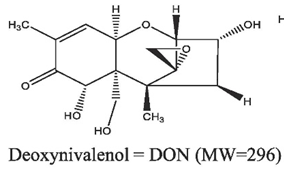
\includegraphics[width=0.25\textwidth]{Images/fig_1.png}
    \caption{Formule semi développée du Deoxynivalenol, molécule de la famille des B-trichothécènes produite par les \textit{Fusarium}\cite{gaballah2023development}}
    \label{fig:mol}
\end{SCfigure}

Jusqu’à présent, le processus de production des mycotoxines a été étudié en ne considérant "qu’un pathogène - une maladie". Cependant, des preuves irréfutables des interactions entre les espèces de \textit{Fusarium} responsables de la fusariose, laisse suggérer que la communication entre ces champignons puisse moduler la régulation de production des toxines.\\

Afin de mettre en exergue les mécanismes de production de ces molécules inter-individus, il est nécessaire changer d'échelle d'analyse afin d’observer plus globalement le "Meta-Fusarium sp." qui comprend les principales espèces impliquées dans l’infection.\cite{ponts2009fusarium, mycsa} \\

\begin{SCfigure}[1][h]
    \centering
    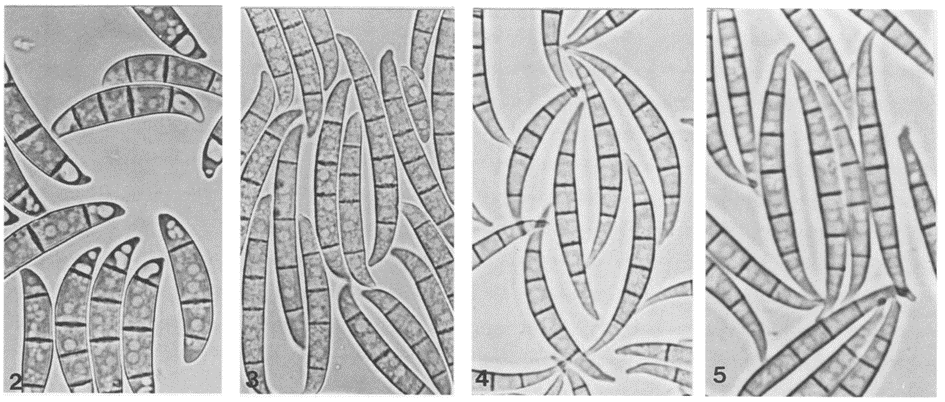
\includegraphics[width=.40\textwidth]{Images/fig_2.png}
    \caption{Observation 5 : de macroconidies de \textit{F.graminearum} (950X), 9 : de microcondies de \textit{F.verticillioides} (avant \textit{F.moniliforme} \cite{name}) (1000X) qui sont des champignons qui font partie du Meta-\textit{Fusarium sp.}.  \cite{taxonomy}}
    \label{fig:fusa}
\end{SCfigure}

\subsection{Communication au sein du Meta-
\textit{Fusarium sp.}}
Au sein du Meta-\textit{Fusarium sp.}. la communication s’effectue en partie par le biais de petits acides ribonucléiques comme les small ARN (smRNA) ou les micro ARN (miRNA). Ces derniers sont des courtes séquences de bases non codantes qui peuvent être séquencées.\\

\begin{figure}[h]
    \centering
    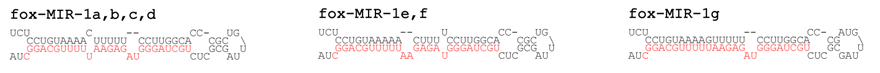
\includegraphics[width=1\textwidth]{Images/fig_3.png}
    \caption{Structure secondaire de quelques précurseurs miARN déjà mis en évidence chez les champignons du genre \textit{Fusarium}.\cite{chen2014exploring}}
    \label{fig:mirna}
\end{figure}

Ces petites molécules d'ARN non codantes d'environ 22 nucléotides, sont impliqués dans la régulation post-transcriptionnelle de l'expression génique. En identifiant les miARN spécifiquement produits lors de la communication induite par la rencontre entre deux Fusaria de la même souche, nous pourrons mieux comprendre les mécanismes sous-jacents aux interactions entre les espèces de \textit{Fusarium} toxinogènes. Et ainsi, développer des stratégies de prévention contre la contamination des cultures par les champignons \textit{Fusarium}. \cite{ponts2009fusarium, mycsa} \\

L’objectif du projet est d’analyser les données séquencées et d’identifier les microARN produits dans chaque scénario de culture, d’en repérer les spécificités et de les quantifier.

\section{État de l'art}

\subsection{Contrôle qualité des reads}
Contrôle qualité des fichiers fastQ pour supprimer ou modifier les artéfacts et les reads de mauvaise qualité.Utilisation de logiciels tels que FastQC.\\

FastQC est un outil utilisé pour évaluer rapidement la qualité des données de séquençage. Il fournit des statistiques détaillées et des graphiques pour identifier les problèmes potentiels tels que la qualité des bases, la distribution des tailles d'insertion, la présence d'adaptateurs, etc.
FastQC est souvent utilisé comme première étape dans l'analyse des données de séquençage pour évaluer rapidement la qualité globale des échantillons. Il est gratuit est disponible sur Github.\cite{fastqc} \\

Il existe un autre outil utilisé MultiQC \cite{multiqc} qui est un outil qui permet d'agréger les résultats de plusieurs analyses FastQC (ou d'autres outils similaires) en un seul rapport. MultiQC est particulièrement pratique lorsque vous effectuez une analyse à grande échelle impliquant de nombreux échantillons, car il permet de consolider les résultats de manière efficace. \\

Le choix entre FastQC et MultiQC dépend de notre besoin d'une évaluation détaillée de la qualité des données pour chaque échantillon individuel, ce qui signifie que FastQC est souvent le meilleur choix.\\

Le QC doit être effectué à deux moments cruciaux : avant et après le nettoyage des données. L'utilisation de MultiQC peut illustrer les différences de qualité avant et après le nettoyage, permettant une évaluation précise de l'efficacité des procédures de nettoyage. Les métriques de qualité attendues en sortie de QC comprennent le nombre de séquences initiales, le nombre après nettoyage, le pourcentage d'ARN ribosomique (rRNA), le pourcentage d'ARN de petite taille (15-17 nt) qui peuvent indiquer la présence de produits de dégradation, le pourcentage de séquences de moins de 15 nt, et la distribution des tailles des miARN (par exemple, 21, 22, 23 nt). Ces métriques fournissent des indicateurs essentiels de la qualité des données et de l'efficacité du nettoyage, facilitant l'optimisation des étapes subséquentes du processus d'analyse. \\

\noindent Sorties attendues :
\begin{itemize}
    \item Statistiques détaillées sur la qualité des données de séquençage
    \item Graphiques pour identifier les problèmes potentiels tels que la qualité des bases, la distribution des tailles d'insertion, la présence d'adaptateurs, etc.
    \item Format de sortie : Rapport HTML généré par FastQC.
\end{itemize}


\subsection{Nettoyage des reads}
Pour le nettoyage des lectures (reads) de séquençage, deux outils principaux se distinguent :  Trimmomatic \cite{trimmomatic} et  Cutadapt \cite{martin2011cutadapt}.\\

Tandis que Cutadapt est reconnu pour son efficacité à éliminer les adaptateurs et les bases de faible qualité, Trimmomatic offre une solution complète pour le nettoyage des lectures, incluant la suppression des adaptateurs, la coupe des bases de faible qualité, et l'élimination des lectures de mauvaise qualité à partir des extrémités. \\

Cutadapt est un outil performant destiné au nettoyage des séquences en éliminant les adaptateurs, les bases de faible qualité, ainsi que les séquences de mauvaise qualité des extrémités des lectures (reads). Il se distingue par sa spécialisation dans la détection et la suppression efficace des séquences d'adaptateurs. Cette spécificité fait de Cutadapt un choix privilégié pour les projets nécessitant une élimination précise et efficiente des adaptateurs.\\

Cutadapt génère des fichiers de séquences nettoyées, optimisant ainsi les données pour l'alignement ou d'autres types d'analyses subséquentes. Sa réputation s'appuie sur sa flexibilité et sa capacité à s'adapter à divers besoins spécifiques de nettoyage de séquences, rendant souvent Cutadapt plus simple à configurer et à utiliser par rapport à Trimmomatic pour certains projets.\\

\noindent Paramètres recommandés pour Cutadapt :
\begin{itemize}
    \item Élimination des adaptateurs : Spécifiez les séquences d'adaptateurs à éliminer. Par exemple, -a ADAPTATEUR pour les adaptateurs en 3' ou -g ADAPTATEUR pour ceux en 5'.
    \item Qualité minimum : Utilisez -q QUALITÉ, pour couper les bases de faible qualité des extrémités des reads. QUALITÉ doit être remplacée par le score de qualité souhaité, comme -q 20 pour supprimer les bases ayant un score de qualité inférieur à 20.
    \item Longueur minimale : Définissez la longueur minimale d'un read pour être conservé avec -m LONGUEUR, où LONGUEUR est la taille minimale requise. Les reads plus courts que cette valeur seront éliminés.
    \item Recadrage : Si nécessaire, vous pouvez recadrer les reads à une longueur spécifique avec -l LONGUEUR, garantissant que tous les reads ont une taille uniforme après le traitement.
\end{itemize} \vspace{.5cm}

\noindent Sorties attendues :
 \begin{itemize}
     \item Fichiers de sortie contenant les reads nettoyés
     \item Format de sortie : Fichiers FASTQ prêts à être utilisés pour l'alignement ou d'autres analyses.
 \end{itemize} \vspace{.5cm}
 
En conclusion, bien que Trimmomatic soit un outil puissant pour le nettoyage des lectures de séquençage, Cutadapt a été choisi pour sa spécialisation dans l'élimination des adaptateurs, sa facilité d'utilisation, et sa capacité à être finement ajusté pour répondre aux besoins spécifiques de notre projet.
 
\subsection{Alignement des reads sur le génome}
Pour ce projet qui se concentre sur l'analyse des petits ARNs (smRNA) non codants, environ 22 nucléotides de long, issus de co-cultures de céréales et de champignons du genre Fusarium, la sélection de l'outil d'alignement est cruciale pour identifier précisément les origines et les cibles potentielles de ces smRNAs dans les génomes des protagonistes. Les caractéristiques clés de ce projet—la courte longueur des séquences d'intérêt et la nécessité de distinguer finement les smRNAs spécifiques à chaque espèce dans des contextes de co-culture orientent vers certains critères pour le choix de l'outil d'alignement :

\begin{itemize}
    \item Sensibilité et précision à aligner de courtes séquences : Étant donné la petite taille des smRNAs, l'outil d'alignement doit être optimisé pour aligner de très courtes séquences de manière précise.
    \item Capacité à gérer des séquences multimappées : Les smRNAs peuvent avoir des séquences qui s'alignent sur plusieurs régions du génome, rendant essentielle la capacité de l'outil à traiter efficacement les lectures multimappées.
    \item Performance et efficacité : Le traitement rapide des données est crucial, surtout lorsqu'on travaille avec un grand nombre d'échantillons typique des analyses à grande échelle.
\end{itemize} \vspace{.5cm}

En considérant ces critères, BWA-MEM2\cite{bwamem2} semble être un choix judicieux pour ce projet. BWA-MEM2 est une version améliorée de BWA-MEM, connue pour son efficacité dans l'alignement de séquences courtes et longues. Ses avantages sont particulièrement pertinents ici :

\begin{itemize}
    \item Haute performance : BWA-MEM2 est optimisé pour les architectures de processeur modernes, offrant une vitesse d'alignement supérieure, ce qui est bénéfique pour traiter rapidement de grands jeux de données.
    \item Précision avec les courtes lectures : Bien que BWA-MEM (et par extension, BWA-MEM2) soit conçu pour être polyvalent, sa capacité à aligner précisément de courtes séquences en fait un choix adapté pour l'analyse de smRNAs.
    \item Gestion des lectures multimappées : BWA-MEM2 offre des options pour ajuster la manière dont les lectures multimappées sont traitées, permettant une analyse fine qui est essentielle pour distinguer les smRNAs provenant de différentes sources dans les co-cultures.
\end{itemize} \vspace{.5cm}

D'autre part,   Bowtie2 \cite{bowtie2} est un outil de cartographie de reads à haut débit qui aligne efficacement les reads sur un génome de référence en utilisant l'algorithme de l'alignement parfaite. Il génère des fichiers d'alignement indiquant où chaque read s'aligne sur le génome de référence.
Sorties attendues :
\begin{itemize}
    \item Fichiers d'alignement indiquant où chaque read s'aligne sur le génome de référence
    \item Format de sortie : Fichiers SAM ou BAM.
\end{itemize} \vspace{.5cm}

En résumé, BWA-MEM2 est recommandé pour sa performance globale et sa capacité à traiter efficacement des séquences courtes et complexes comme celles rencontrées dans ce projet. 

\subsection{Identification des petits ARN produits }
L'étape cruciale suivant l'alignement des données de séquençage de petits ARN (smRNA-seq) est l'identification et l'annotation des microARNs (miARNs) présents dans chaque échantillon, provenant de diverses situations de co-culture. Pour cela, deux outils principaux sont utilisés : miRDeep2\cite{friedlander2012discover} et miRBase \cite{kozomara2019mirbase}, chacun ayant un rôle spécifique dans le processus d'analyse.\\ 

\begin{itemize}
    \item Utilisation de miRDeep2:
    miRDeep2 est un outil de bioinformatique conçu spécialement pour l'identification et la prédiction de nouveaux miARNs à partir des données de séquençage de smRNA. Il fonctionne en intégrant les séquences de smRNA alignées avec des informations sur la structure secondaire des précurseurs de miARN pour prédire de nouveaux miARNs et évaluer leur probabilité. Cette capacité à découvrir de nouveaux miARNs le rend particulièrement utile pour les recherches exploratoires où l'identification de miARNs inconnus peut fournir des insights novateurs sur les mécanismes moléculaires sous-jacents à l'interaction entre les espèces dans les co-cultures.
    \item Rôle de miRBase:
    En contraste, miRBase sert de base de données de référence exhaustive pour les séquences de miARNs déjà connues et annotées. Cet outil est crucial pour l'annotation des séquences de miARN détectées dans les échantillons de séquençage, permettant de relier les séquences observées à des fonctions et des rôles biologiques établis. L'utilisation de miRBase est essentielle pour distinguer les miARNs nouvellement découverts des séquences déjà documentées, facilitant ainsi la détermination de leur potentiel biologique et fonctionnel.
    \item Approche combinée:
    Pour une analyse complète des données de smRNA-seq issues de co-cultures, une approche combinée qui utilise à la fois miRDeep2 pour la découverte de nouveaux miARNs et miRBase pour l'annotation des miARNs connus est recommandée. Cette stratégie permet de maximiser la couverture analytique, offrant à la fois la possibilité de découvrir de nouvelles entités régulatrices et de relier les miARNs détectés à des connaissances biologiques existantes. Ce processus d'identification et d'annotation est fondamental pour comprendre les mécanismes moléculaires par lesquels les petits ARN facilitent la communication entre les espèces dans les co-cultures, ouvrant la voie à des stratégies de prévention des contaminations par des mycotoxines dans les céréales.
\end{itemize} \vspace{.5cm}

\noindent Sorties attendues :
\begin{itemize}
    \item Liste des miARN identifiés dans chaque échantillon
    \item Format de sortie : Rapport ou fichier texte.
\end{itemize}

\subsection{Quantification des petits ARN }
L'étape de quantification de l'expression des petits ARN repose sur l'évaluation des niveaux d'expression des séquences identifiées, en s'appuyant sur des outils spécialisés tels que HTSeq\cite{anders2015htseq} ou featureCounts \cite{liao2014featurecounts}. Ces outils analysent les données de séquençage d'ARN à petite échelle pour estimer l'abondance des ARN dans les échantillons.\\

L'analyse inclura notamment la quantification des ARN ribosomaux et la détermination de leur distribution et abondance relative dans les échantillons.\\

\begin{itemize}
    \item Utilisation de HTSeq:
    HTSeq est un outil développé en Python, spécialement conçu pour traiter les données issues de séquençage à haut débit, y compris les données de séquençage de petits ARN. Il fonctionne en prenant les lectures séquencées alignées (au format BAM) et les compare à un fichier d'annotation de référence pour attribuer chaque lecture à une caractéristique génomique spécifique, telle que les gènes ou les petits loci d'ARN.
    \item Fonctionnalités de featureCounts:
    D'autre part, featureCounts, qui fait partie intégrante du package Subread, est également utilisé pour cartographier et quantifier les lectures de séquences. Comme HTSeq, featureCounts utilise des lectures alignées et un fichier d'annotation pour assigner les lectures à des caractéristiques génomiques définies. L'outil génère une matrice de comptage où chaque ligne représente une caractéristique génomique (par exemple, un petit ARN) et chaque colonne un échantillon, affichant le nombre de lectures mappées à chaque caractéristique pour chaque échantillon. Une fonctionnalité clé de featureCounts est sa capacité à effectuer le comptage de lectures spécifique à un brin, une propriété essentielle pour la quantification précise des petits ARN, surtout en considération de la transcription antisens.
    \item Choix entre HTSeq et featureCounts:
    Pour ce projet, où la distinction précise entre les petits ARN issus des co-cultures est critique, featureCounts est privilégié en raison de sa capacité à effectuer des quantifications spécifiques à un brin. Cette fonctionnalité est particulièrement pertinente pour les petits ARN, dont l'orientation peut être cruciale pour leur fonction biologique et leur identification correcte. La précision dans la quantification de l'expression des petits ARN est fondamentale pour analyser leur rôle dans la communication inter-espèces.
\end{itemize} \vspace{.5cm}

\noindent Sorties attendues :
\begin{itemize}
    \item Matrice de comptage des lectures de séquences attribuées à chaque caractéristique génomique dans chaque échantillon
    \item Format de sortie : Matrice de comptage (par exemple, format texte ou tableur).
\end{itemize}

\subsection{Normalisation}
L’objectif principal de la normalisation est d’ajuster les différences de profondeur de séquençage et les biais de composition entre les échantillons. Ceci est essentiel pour une analyse précise en aval, en particulier lors de la comparaison des niveaux d’expression entre échantillons ou conditions.
EdgeR\cite{robinson2010edger} et DESeq2\cite{love2014moderated} proposent tous deux des méthodes de normalisation largement utilisées dans l’analyse de séquençage d’ARN. Ces outils utilisent des modèles statistiques pour tenir compte des effets de profondeur de lecture et de composition d’ARN. \\

\begin{itemize}
    \item EdgeR : Utilise une méthode basée sur l'échelle des tailles de bibliothèque normalisées. La fonction calcNormFactors dans EdgeR calcule des facteurs d'échelle pour chaque bibliothèque qui sont ensuite utilisés pour ajuster les comptages de lecture.
    DESeq2 : Fournit une méthode de normalisation des facteurs de taille qui est calculée en utilisant la méthode de médiane des ratios. Cela permet d'ajuster simultanément la profondeur de séquençage et la composition d'ARN.
    \item Sorties attendues :les données lues de séquençage réelles représentées au format BAM ne sont pas modifiées en termes de normalisation. La normalisation affecte généralement la façon dont vous interprétez les données (comme l'ajustement du nombre de lectures dans l'analyse), et non les lectures brutes elles-mêmes.
\end{itemize}

\subsection{Analyse différentielle}
Identification des petits ARN différentiellement exprimés entre les différentes conditions de co-culture à l'aide d'outils comme DESeq2 \cite{love2014moderated} ou edgeR\cite{robinson2010edger}.\\

\begin{itemize}
    \item Utilisation de DESeq2 et edgeR
    DESeq2 et edgeR sont des packages de bioinformatique conçus spécifiquement pour analyser les variations d'expression génique ou, dans ce cas, des petits ARN, à partir de données de séquençage d'ARN. Ces outils appliquent des modèles statistiques pour identifier les caractéristiques génomiques—ici, les petits ARN—qui montrent des changements d'expression significatifs entre les conditions expérimentales étudiées. DESeq2 utilise un modèle basé sur les négatives binomiales pour estimer la variance et la moyenne des données d'expression, permettant une comparaison précise entre les groupes. EdgeR, de son côté, emploie également une approche basée sur les négatives binomiales, avec une emphase sur la normalisation des tailles d'échantillons et une estimation robuste de la dispersion pour identifier les différences d'expression.
    \item Vérification de la validité de l'approche:
    L'adéquation de DESeq2 ou edgeR pour l'analyse différentielle des petits ARN dans le contexte des co-cultures de céréales et Fusarium dépend de plusieurs facteurs, notamment la normalisation appropriée des données et la précision dans l'estimation de la dispersion. Ces facteurs sont cruciaux étant donné la complexité des interactions et le potentiel de variation entre les échantillons.
\end{itemize} \vspace{.5cm}

\noindent Sorties attendues :
\begin{itemize}
    \item Liste des miARN différentiellement exprimés avec leur niveau de significativité statistique
    \item Format de sortie : Tableau ou fichier texte.
\end{itemize}

\subsection{Visualisation des résultats}
Matplotlib, en tant que bibliothèque de visualisation de données pour Python, offre une flexibilité et une variété d'options pour présenter ces données de manière informative et visuellement attrayante. Voici quelques types de visualisations spécifiquement adaptées à l'analyse de séquençage de petits ARN qui pourraient être envisagées :
\begin{itemize}
    \item Histogrammes de distribution
    \item Graphiques en boîte (Boxplots)
    \item Graphiques de dispersion (Scatter plots)
    \item Heatmaps
    \item Diagrammes de Volcano
\end{itemize} \vspace{.5cm}

\noindent Sorties attendues :
\begin{itemize}
    \item Graphiques représentant les résultats de l'analyse de séquençage
    \item Format de sortie : Graphiques (par exemple, fichiers image ou intégration dans un rapport).
\end{itemize} \vspace{.5cm}

Le pipeline sera livré sous la forme de scripts Python, éventuellement accompagnés de fichiers de configuration ou de documentation supplémentaire. Ces scripts seront conçus pour être exécutés de manière séquentielle ou modulaire, selon les besoins de l'utilisateur.\\

En ce qui concerne le dépôt, GitHub est souvent utilisé comme plateforme populaire pour héberger des projets de développement logiciel. Nous pourrions créer un référentiel GitHub dédié pour stocker le code source du pipeline, ainsi que toute documentation supplémentaire ou des exemples d'utilisation. Cela permettra aux utilisateurs de télécharger facilement le pipeline, de suivre les mises à jour et de contribuer au développement si nécessaire.

\section{Analyse des besoins}

\subsection{Besoins fonctionnels}
Pour le prétraitement des données, les besoins comprennent :
\begin{itemize}
    \item Acquisition des données issues du séquençage Illumina (Short Read) générées à partir de différentes conditions de culture de Fusarium au format FASTQ.
    \item Prétraitement et nettoyage des données brutes afin d'éliminer les séquences de faible qualité et les erreurs techniques en réalisant un contrôle qualité des lectures.
    \item Normalisation des données.
\end{itemize}

Pour l'analyse des données, les besoins incluent :  
\begin{itemize}
 \item Alignement des lectures prétraitées sur les génomes de référence des souches de Fusarium.
    \item Identifier les miARNs, déterminer leur origine ou leur localisation génomique, et évaluer leur quantité.
    \item Analyse comparative des profils d'expression des microARN entre les échantillons de cultures pures et ceux des confrontations entre souches.
    \item Visualisation des résultats à travers des tableaux et des graphiques codifiés présentant les profils d'expression des miARNs dans les différentes conditions de culture.
\end{itemize}

\subsection{Besoins non fonctionnels}
\begin{itemize}
    \item Utilisation recommandée des langages de programmation adaptés à la bioinformatique, tels que Python, R et éventuellement Bash.
    \item Traitement efficace des données dans des délais raisonnables.
    \item Fiabilité et robustesse pour minimiser les risques de perte de données ou d'erreurs dans l'analyse.
    \item Intuitivité pour une utilisation aisée par les chercheurs non spécialisés en bioinformatique.
    \item Documentation claire et interfaces rationnelles pour faciliter la navigation et l'utilisation des fonctionnalités.
\end{itemize}

\subsection{Contraintes}
\begin{itemize}
    \item Utiliser des outils open source afin d'assurer la transparence, la réutilisabilité du système.
    \item Effectuer nos tâches dans un cadre à accès pseudo-restreint.
    \item Sortir un fichier BigWig compatible avec les plates-formes de navigateur de génome fonctionnelles existantes comme JBrowse pour garantir une visualisation adéquate.
\end{itemize}

\subsection{Ajouts optionnels}
\begin{itemize}
    \item Création d'une base de données pour stocker les résultats.
    \item Sauvegarde et reprise du processus d'analyse et reprise de l'analyse là où elle s'est arrêtée.
    \item Identification des cibles potentielles des miARNs dans les génomes des souches.
\end{itemize}

\chapter{Flux opérationnel}
Voici un diagramme reprenant les différents points à réaliser.
\begin{center}
    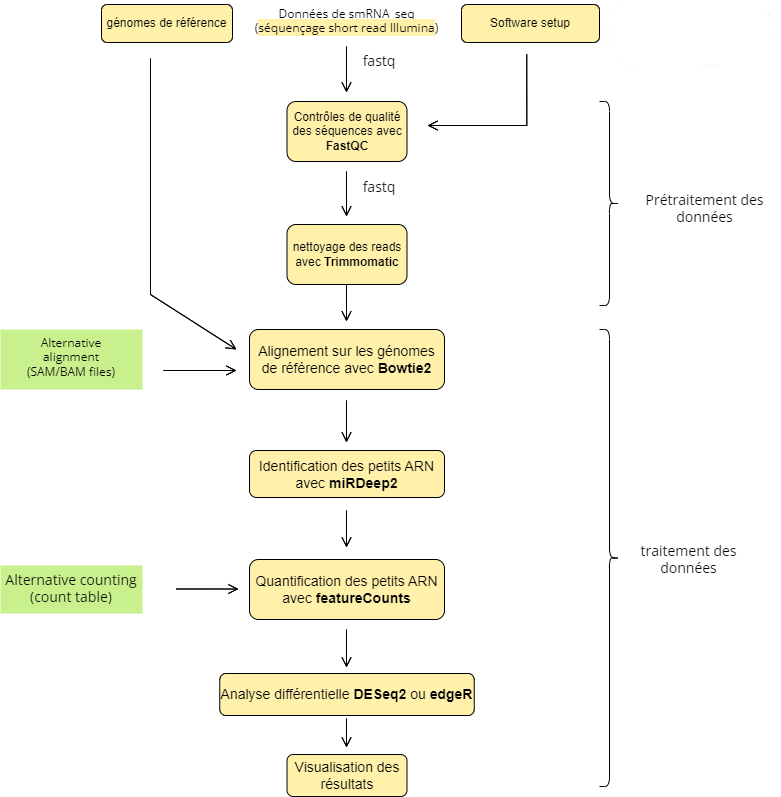
\includegraphics[scale=0.6]{Images/PIPLINE_RNA.png}\\[1cm]
\end{center}

\chapter{Organisation}
\section{Diagramme de Gantt}
\begin{figure}[h]
    \centering
    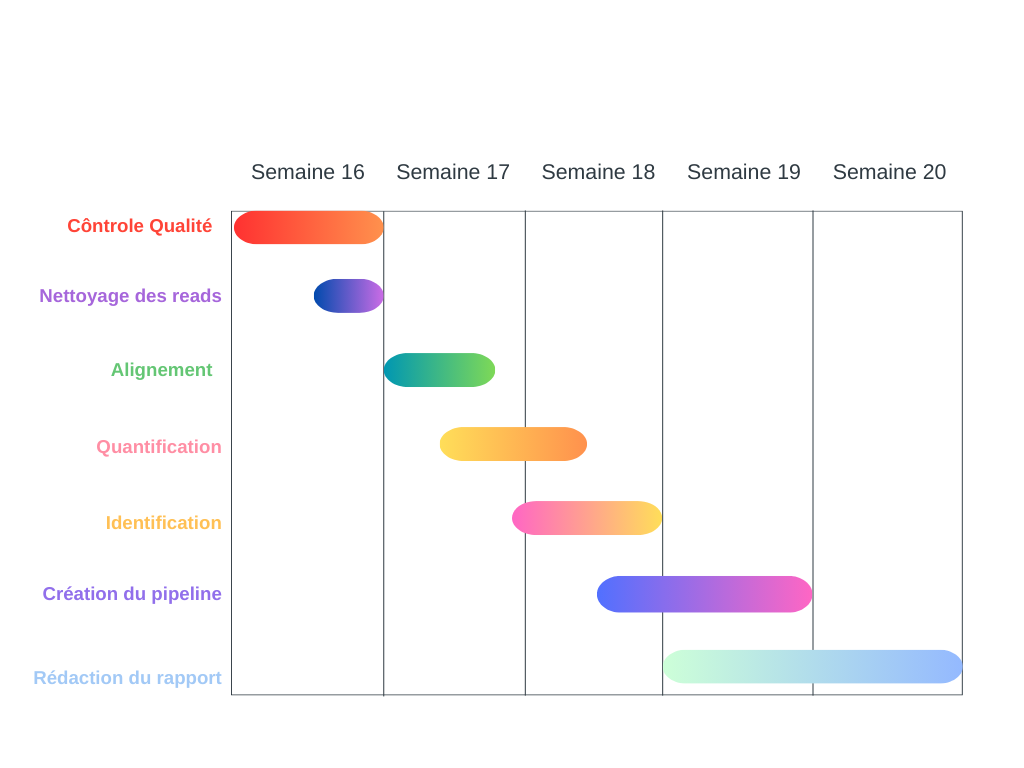
\includegraphics[width=0.8\textwidth]{Images/controle_qual.png}
    \caption{Diagramme de Gantt qui nous servira de base pour l'organisation de notre travail}
    \label{fig:enter-label}
\end{figure}

\bibliography{biblio}

\end{document}
